\documentclass{../../slides-style}

\slidetitle{Сборка и непрерывная интеграция}{12.09.2023}

\begin{document}

    \begin{frame}[plain]
        \titlepage
    \end{frame}

    \section{Системы сборки}

    \begin{frame}
        \frametitle{Системы сборки}
        \begin{itemize}
            \item Среда разработки не всегда доступна
            \begin{itemize}
                \item Continuous Integration-сервера автоматически выполняют сборку после каждого коммита, там некому открыть IDE и нажать на кнопку ``запустить''
            \end{itemize}
            \item Воспроизводимость сборки
            \begin{itemize}
                \item Если чтобы собрать программу надо открыть проект, скопировать пару десятков файлов, поправить кое-какие пути и делать это в полнолуние, то возможны ошибки
            \end{itemize}
            \item Автоматизация сборки
            \begin{itemize}
                \item git clone
                \item одна консольная команда, которая всё делает за нас
                \item ...
                \item готовое к работе приложение
            \end{itemize}
        \end{itemize}
    \end{frame}

    \begin{frame}[fragile]
        \frametitle{Сборка вручную без IDE}
        \begin{itemize}
            \item gcc
            \begin{footnotesize}
                \begin{minted}{text}
    g++ <имя .c-файла>
                \end{minted}
            \end{footnotesize}
            или, например,
            \begin{footnotesize}
                \begin{minted}{text}
    g++ -Wall -o helloworld helloworld.c
                \end{minted}
            \end{footnotesize}
            \item Если проект большой, это быстро становится грустно
            \begin{itemize}
                \item Десятки тысяч файлов --- не редкость
            \end{itemize}
        \end{itemize}
    \end{frame}

    \begin{frame}
        \frametitle{make}
        \begin{itemize}
            \item Стандарт де-факто по ``низкоуровневым'' правилам сборки
            \item Сама ничего не знает про языки программирования, компиляторы и прочие подобные штуки
            \item Знает про цели, зависимости, временные штампы и правила
            \begin{itemize}
                \item Смотрит на зависимости цели, если у хоть одной временной штамп свежее цели, запускается правило для цели
                \item В процессе цель может обновить свой временной штамп, что приведёт к исполнению правил для зависящих от неё целей
                \item Цели и зависимости образуют направленный ациклический граф (DAG)
                \item make выполняет топологическую сортировку графа зависимостей
                \item Правила применяются в порядке от листьев к корню
            \end{itemize}
            \item Правила сборки описываются в Makefile
        \end{itemize}
    \end{frame}

    \begin{frame}[fragile]
        \frametitle{Пример}
        \begin{footnotesize}
            \begin{minted}{make}
target [target ...]: [component ...]
    [command 1]
    .
    .
    .
    [command n]
            \end{minted}
        \end{footnotesize}
        Пример:
        \begin{footnotesize}
            \begin{minted}{text}
hello: ; @echo "hello"
            \end{minted}
        \end{footnotesize}
    \end{frame}

    \begin{frame}
        \frametitle{Высокоуровневые системы сборки}
        \begin{itemize}
            \item C/C++:
            \begin{itemize}
                \item CMake --- кроссплатформенная система сборки, очень популярна в C++ open source-сообществе
                \item MSBuild --- система сборки Visual Studio
                \item qmake, qbs --- системы сборки от фреймворка Qt
            \end{itemize}
            \item JVM:
            \begin{itemize}
                \item Maven --- старая, но популярная и ``архитектурно правильная''
                \item Gradle --- несколько более ``императивна'', нынче более популярна, поддерживает Kotlin
            \end{itemize}
            \item .NET --- dotnet CLI, FAKE
        \end{itemize}
        Написание скриптов сборки для большого проекта --- отдельная и довольно трудоёмкая задача
    \end{frame}

    \section{Continuous Integration}

    \begin{frame}
        \frametitle{Continuous Integration}
        Непрерывная интеграция --- практика слияния всех изменений по нескольку раз в день, сборки их в известном окружении и запуска юнит-тестов.
        \begin{itemize}
            \item Автоматическая сборка
            \begin{itemize}
                \item Всё, что нужно для сборки, есть в репозитории, может быть получено на чистую (ну, практически) машину и собрано одной консольной командой
            \end{itemize}
            \item Большое количество юнит-тестов, запускаемых автоматически
            \item Выделенная машина, слушающая репозиторий и выполняющая сборку
            \begin{itemize}
                \item Чаще всего каждая сборка запускается на заранее настроенной виртуалке или в Docker-контейнере
            \end{itemize}
        \end{itemize}
    \end{frame}

    \begin{frame}
        \frametitle{Continuous Integration}
        \begin{itemize}
            \item Извещение всех разработчиков о статусе
            \begin{itemize}
                \item Если билд не прошёл, разработка приостанавливается до его починки
            \end{itemize}
            \item Автоматическое выкладывание
            \item Пока билд не прошёл, задача не считается сделанной
            \begin{itemize}
                \item Короткие билды (<10 мин.)
                \item deployment pipeline
                \begin{itemize}
                    \item Отдельная машина для сборки, для коротких тестов, для длинных тестов, для выкладывания
                \end{itemize}
            \end{itemize}
        \end{itemize}
    \end{frame}

    \section{GitHub Actions}

    \begin{frame}
        \frametitle{GitHub Actions}
        \begin{itemize}
            \item Бесплатная система облачной сборки для проектов на GitHub
            \item \url{https://docs.github.com/en/actions}
            \item Как настроить:
            \begin{itemize}
                \item В репозитории на GitHub Settings -> Actions -> Allow all actions
                \item Создаём в корне репозитория папку .github/workflows/
                \item В нём создаём файл <имя действия>.yml (например, ci.yml)
                \item Описываем процесс сборки согласно \url{https://docs.github.com/en/actions/learn-github-actions/workflow-syntax-for-github-actions}
                \begin{itemize}
                    \item Пример и описание линуксовой сборки: \url{https://www.incredibuild.com/blog/using-github-actions-with-your-c-project}
                \end{itemize}
                \item Коммитим-пушим
                \item Смотрим статус коммита и пуллреквеста
            \end{itemize}
        \end{itemize}
    \end{frame}

    \begin{frame}
        \frametitle{Что получится}
        \begin{center}
            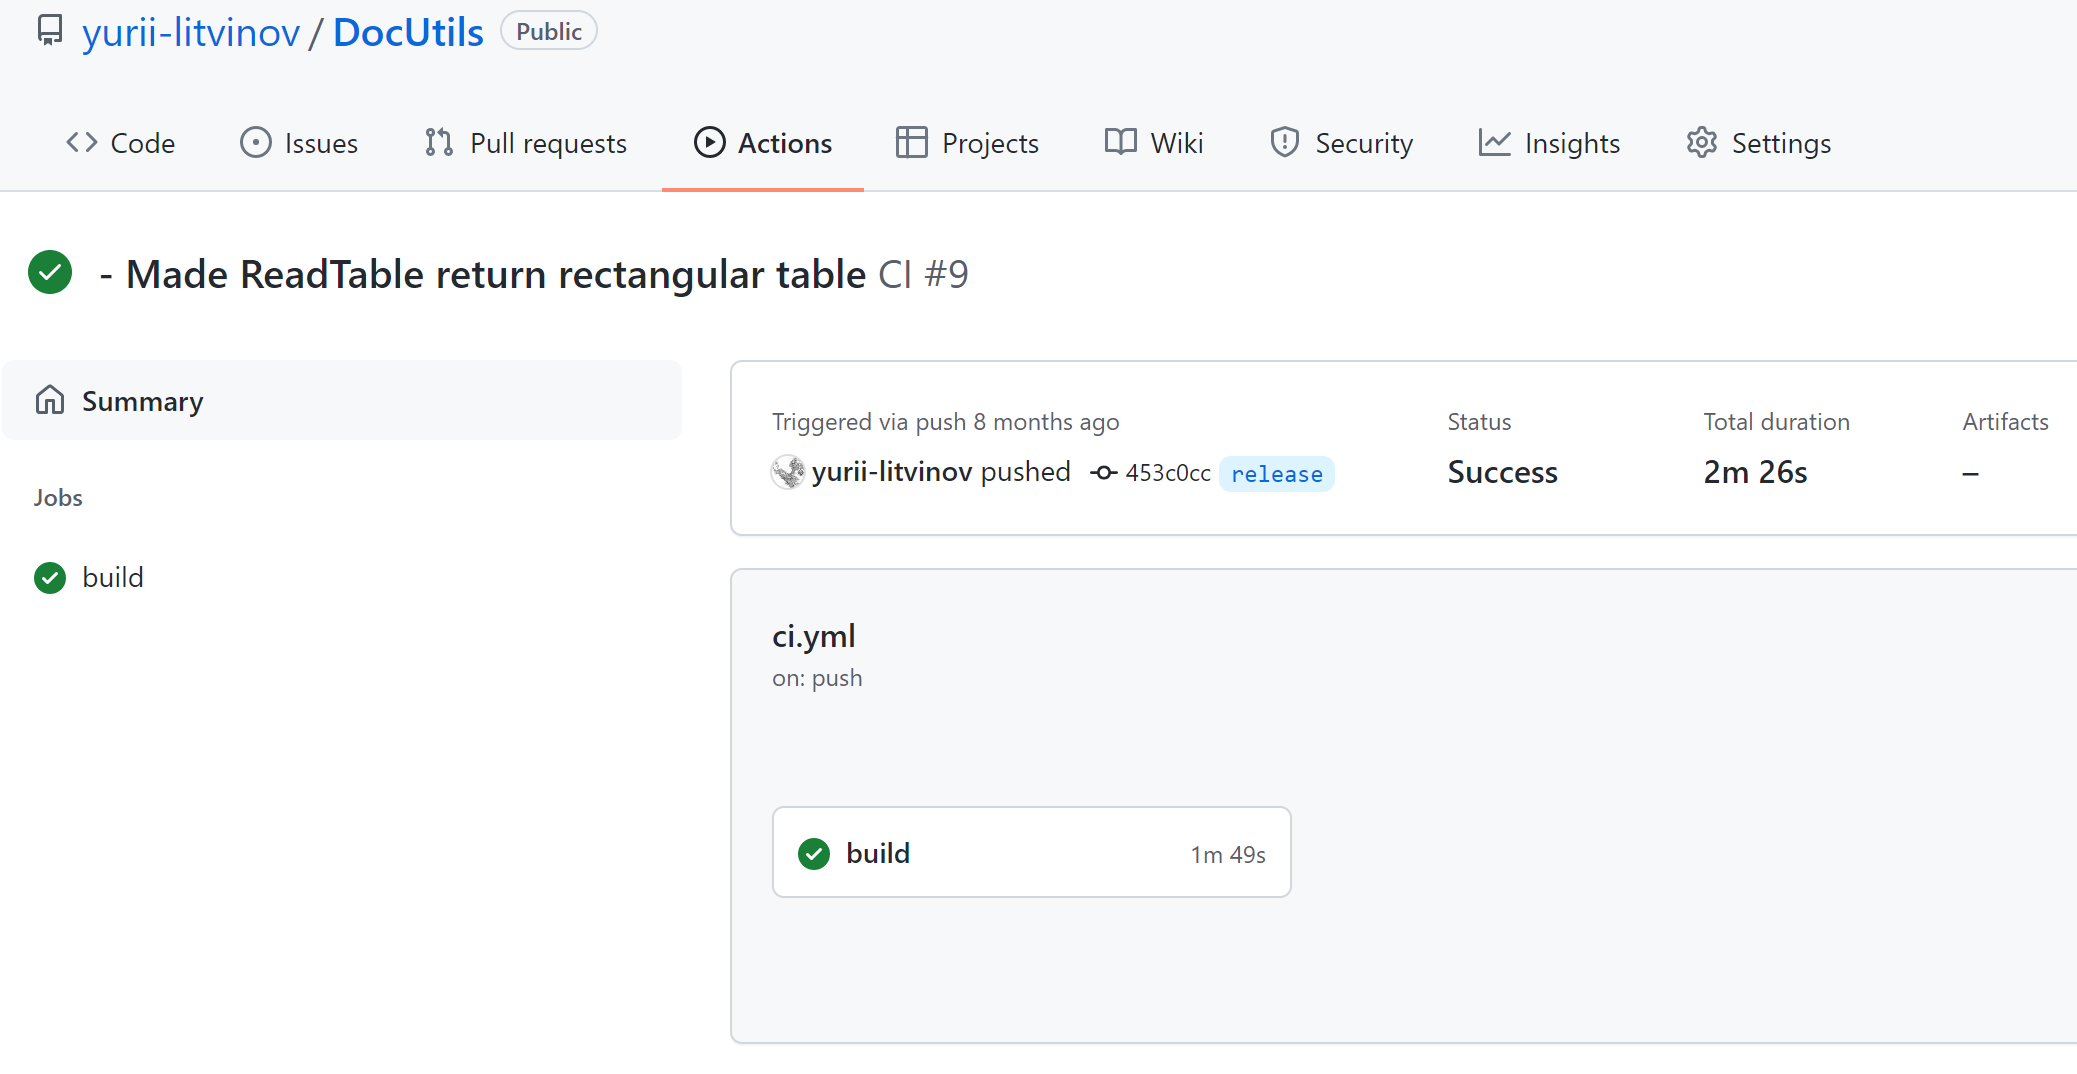
\includegraphics[width=0.9\textwidth]{githubActionsBuildStatus.png}
        \end{center}
        И появятся иконки статуса рядом с коммитами и пуллреквестами
    \end{frame}

    \begin{frame}[fragile]
        \frametitle{Типичный Workflow для сборки}
        \framesubtitle{Java}
        \begin{scriptsize}
            \begin{minted}{yaml}
name: Build
on: [push, pull_request]
jobs:
    build-Ubuntu:
        runs-on: ubuntu-latest
        steps:
            - uses: actions/checkout@v2
            - name: Set up JDK
              uses: actions/setup-java@v1
              with:
                  java-version: 17
            - name: Build
              run: ./gradlew build
            - name: Run tests
              run: ./gradlew test
    build-Windows:
        runs-on: windows-latest
        steps:
                ...
            -   name: Build
                run: .\gradlew.bat build
            -   name: Run tests
                run: .\gradlew.bat test
            \end{minted}
        \end{scriptsize}
    \end{frame}

    \begin{frame}
        \frametitle{GitHub Actions, Workflow и Job}
        \begin{center}
            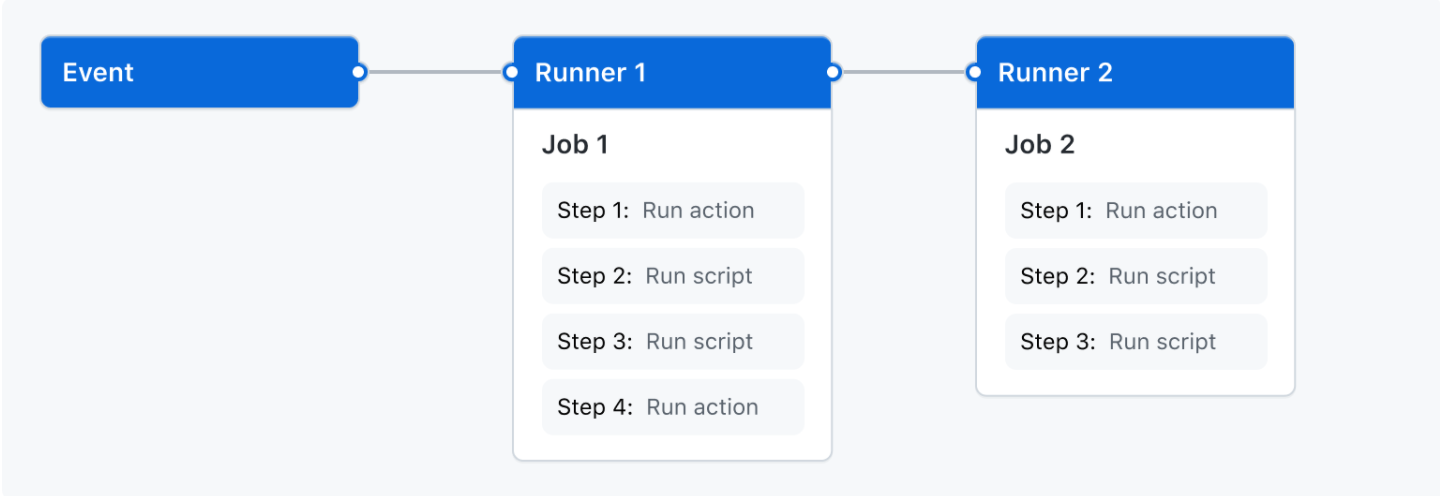
\includegraphics[width=0.7\textwidth]{githubActionsWorkflow.png}
        \end{center}
        \begin{itemize}
            \item Step --- это либо скрипт, либо \emph{Action}
            \item Action --- произвольный код (по сути, отдельное приложение), выполняющийся как шаг Job-а
            \begin{itemize}
                \item Переиспользуемый строительный блок
                \item Можно переиспользовать Workflow-ы
            \end{itemize}
        \end{itemize}
    \end{frame}

    \begin{frame}[fragile]
        \frametitle{Переменные окружения}
        \begin{scriptsize}
            \begin{minted}{yaml}
env:
  DAY_OF_WEEK: Monday

jobs:
  greeting_job:
    runs-on: ubuntu-latest
    env:
      Greeting: Hello
    steps:
      - name: "Say Hello Mona it's Monday"
        if: ${{ env.DAY_OF_WEEK == 'Monday' }}
        run: echo "$Greeting $First_Name. Today is $DAY_OF_WEEK!"
        env:
          First_Name: Mona
            \end{minted}
        \end{scriptsize}
    \end{frame}

    \begin{frame}[fragile]
        \frametitle{Матрица сборки}
        \begin{scriptsize}
            \begin{minted}{yaml}
runs-on: ${{ matrix.os }}
strategy:
  matrix:
    os: [ubuntu-18.04, ubuntu-20.04]
    node: [10, 12, 14]
steps:
  - uses: actions/setup-node@v2
    with:
      node-version: ${{ matrix.node }}
            \end{minted}
        \end{scriptsize}
    \end{frame}

    \begin{frame}
        \frametitle{Что ещё?}
        \begin{itemize}
            \item Секреты
            \begin{itemize}
                \item \mintinline{yaml}|super_secret: ${{ secrets.SUPERSECRET }}|
            \end{itemize}
            \item Кеширование промежуточных результатов
            \item Автоматическое развёртывание
            \begin{itemize}
                \item В том числе, автодеплой документации на github-pages
            \end{itemize}
            \item Проверка стиля кодирования, статический анализ кода и т.п.
            \begin{itemize}
                \item Может быть интересно для Python-разработчиков
            \end{itemize}
            \item Можно иметь несколько Workflow-ов в одном репозитории
        \end{itemize}
    \end{frame}

\end{document}
